\documentclass[10pt,a4paper]{article}
\usepackage{rpgcover} % Loads the original rpgmanual.sty and its fonts
\usepackage{xsavebox}
\RPGSetRunningTitle{The Path of Debts}
\hypersetup{pdftitle={The Path of Debts — At the Last Throw},pdfauthor={Jacopo Biscella}}
\RPGSetCoverWordSpace{.78em}
% Paragraph spacing and leading as in manual-<lang>.tex and the adventure.
\setlength{\parskip}{3pt plus .5pt minus .5pt}
\linespread{1.06}\selectfont
% JPEG copies of the shared cover backgrounds (scripts/build-adventure-print-art.sh), as in the adventure.
\RPGSetFrontBackground{assets/engraved-front-background.jpg}\RPGSetBackBackground{assets/engraved-cover-background.jpg}
% The adventure's front-cover typography, with the overlay saved once (xsavebox) and reused on the
% contents page instead of being embedded twice.
\newcommand{\SentieroFrontCover}{%
 \clearpage\RPGCoverPagetrue\thispagestyle{empty}\null
 \xsavebox{SentieroOverlay}{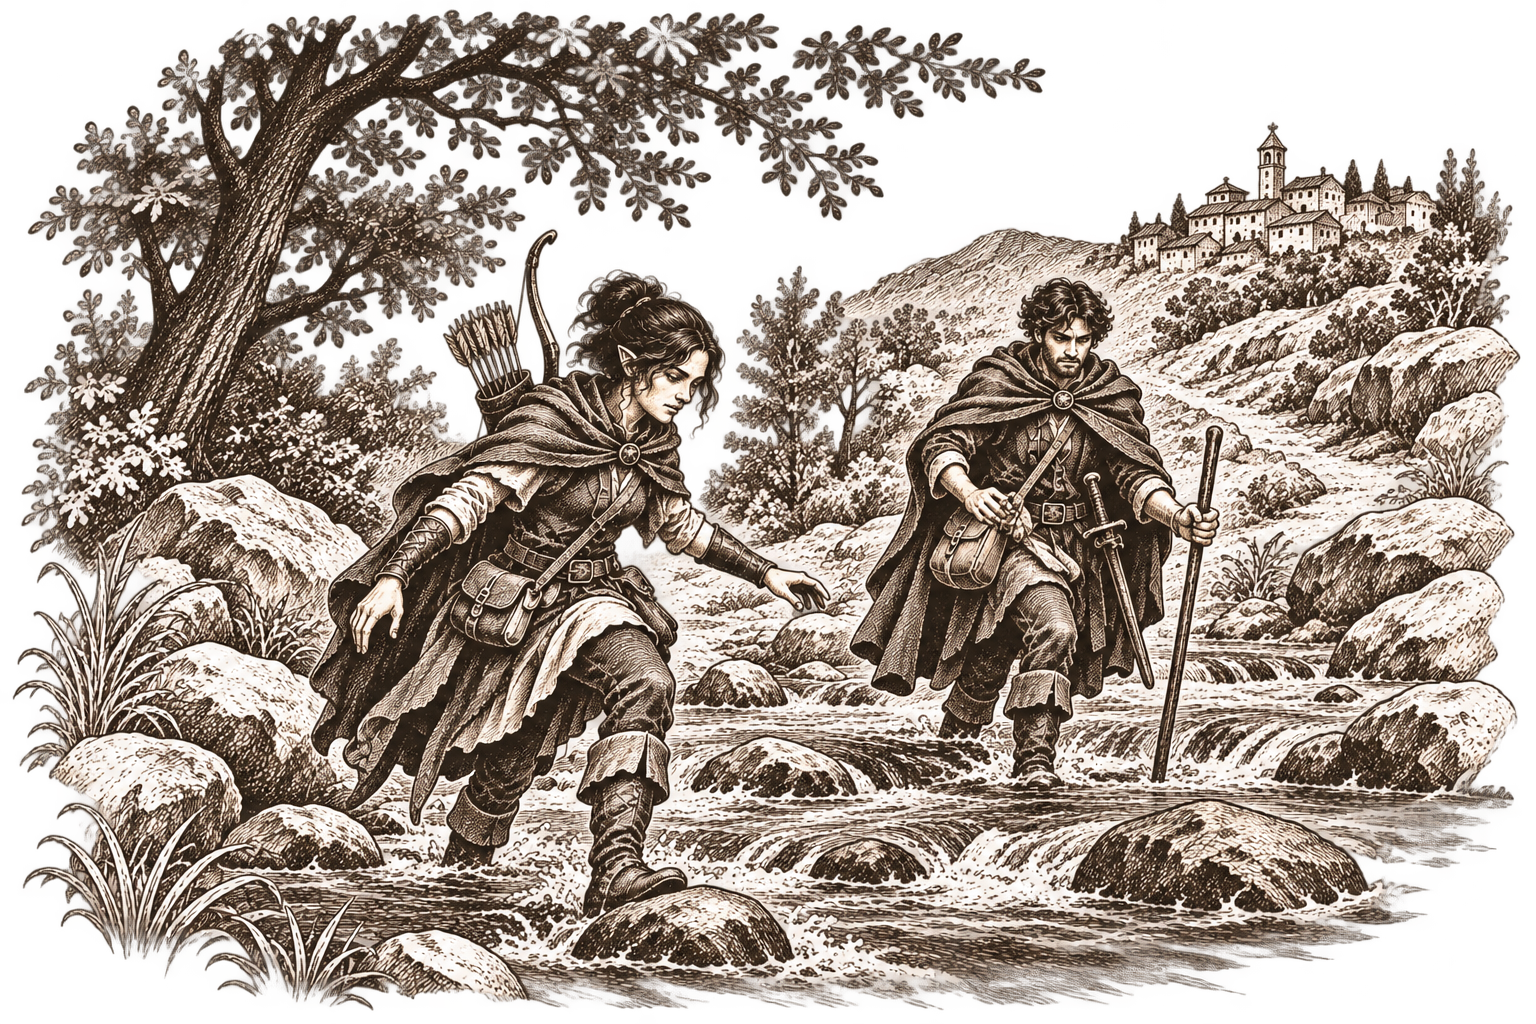
\includegraphics{assets/path-of-debts/front-overlay.png}}%
 \begin{tikzpicture}[remember picture,overlay,x=1mm,y=1mm]
  \RPGDrawBackground{\RPGFrontBackgroundFile}
  % Title and subtitle as on the adventure's cover: same sizes and positions in the cartouche.
  \node[align=center,text=coverink,text width=138mm,inner sep=0pt] at ($(current page.south west)+(105mm,248mm)$)
   {\RPGCoverTitleFont\fontsize{16.6}{20.7}\selectfont\spaceskip=\RPGCoverWordSpace\relax THE PATH\\[1.0mm]OF DEBTS};
  \node[align=center,text=coverink,text width=135mm,inner sep=0pt] at ($(current page.south west)+(105mm,235mm)$)
   {\RPGCoverSubtitleFont\fontsize{9.5}{12}\selectfont An introductory story for “At the Last Throw”};
  \node[inner sep=0pt,anchor=center] at ($(current page.south west)+(105mm,125mm)$)
   {\resizebox{150mm}{!}{\xusebox{SentieroOverlay}}};
  \node[align=center,text=coverink,text width=124mm,inner sep=0pt] at ($(current page.south west)+(105mm,25mm)$)
   {\RPGCoverTextFont\fontsize{12}{15}\selectfont Jacopo Biscella};
 \end{tikzpicture}
 \clearpage\RPGCoverPagefalse}
% Uses precisely the back background and the editable cover fonts from rpgcover.sty.
% This is text layout only: no substitute illustrations or background graphics.
\newcommand{\SentieroBackCover}{%
 \clearpage\pagenumbering{gobble}\RPGCoverPagetrue\thispagestyle{empty}\null
 \begin{tikzpicture}[remember picture,overlay,x=1mm,y=1mm]
   \RPGDrawBackground{\RPGBackBackgroundFile}
   \node[align=center,text=coverink,text width=170mm,inner sep=0pt]
     at ($(current page.south west)+(105mm,260mm)$)
     {{\RPGCoverTitleFont\fontsize{19}{23}\selectfont\spaceskip=\RPGCoverWordSpace\relax THE PATH OF DEBTS}};
   \draw[coverink,line width=.45pt]
     ($(current page.south west)+(57mm,246mm)$)--($(current page.south west)+(153mm,246mm)$);
   % Blocks at the positions of the adventure's back cover: story at 240 mm, small-caps lines at
   % 197, second rule at 167, description at 162, closing line at 133.
   \node[anchor=north,align=left,text=coverink,text width=137mm,inner sep=0pt]
     at ($(current page.south west)+(105mm,240mm)$)
     {\RPGCoverTextFont\fontsize{10.4}{13.4}\selectfont
      A false coin. A letter with no addressee. Two travellers with no reason to trust each other.\par\smallskip
      Nim Thistledown and Mara Veyne follow the King's road to Hollow Hearth. On the way they will learn that a promise can be more dangerous than a weapon, and that some choices have consequences even when no one sees them.};
   \node[anchor=north,align=center,text=coverink,text width=140mm,inner sep=0pt]
     at ($(current page.south west)+(105mm,197mm)$)
     {\RPGCoverSubtitleFont\fontsize{13}{17}\selectfont
      A prologue to “The Bell of Hollow Hearth”};
   \draw[coverink,line width=.45pt]
     ($(current page.south west)+(57mm,167mm)$)--($(current page.south west)+(153mm,167mm)$);
   \node[anchor=north,align=left,text=coverink,text width=137mm,inner sep=0pt]
     at ($(current page.south west)+(105mm,162mm)$)
     {\RPGCoverTextFont\fontsize{10.4}{13.4}\selectfont
      Seven examples show how the players' decisions become rolls, dialogue and consequences at the table of At the Last Throw.};
   \node[anchor=north,align=center,text=coverink,text width=147mm,inner sep=0pt]
     at ($(current page.south west)+(105mm,133mm)$)
     {\RPGCoverSubtitleFont\fontsize{10.5}{13.2}\selectfont
      The story ends where the adventure begins.};
   \filldraw[fill=white,draw=coverink,line width=.55pt]
     ($(current page.south west)+(139mm,25mm)$) rectangle
     ($(current page.south west)+(187mm,55mm)$);
 \end{tikzpicture}
 \clearpage\RPGCoverPagefalse
}
% Dice icons for the "At the table" boxes, drawn with TikZ (no font glyphs, so they work in every
% language). \Dado{n}: a kept d6 showing n; \Dado*{n}: a rolled die that is not kept (faded).
% \Su and \Giu: the rulebook's keep-highest and keep-lowest arrows, from FreeSerif.
% \Bersaglio: the TN to reach. \Riuscita and \Fallita: success and failure.
\newcommand\DadoPips[1]{%
  \ifcase#1\or \fill (.5,.5) circle (.1);
  \or \fill (.27,.73) circle (.1); \fill (.73,.27) circle (.1);
  \or \fill (.25,.75) circle (.09); \fill (.5,.5) circle (.09); \fill (.75,.25) circle (.09);
  \or \foreach \x/\y in {.27/.27,.27/.73,.73/.27,.73/.73}{\fill (\x,\y) circle (.095);}
  \or \foreach \x/\y in {.25/.25,.25/.75,.75/.25,.75/.75,.5/.5}{\fill (\x,\y) circle (.09);}
  \or \foreach \x/\y in {.28/.22,.28/.5,.28/.78,.72/.22,.72/.5,.72/.78}{\fill (\x,\y) circle (.085);}
  \fi}
\makeatletter
\newcommand\Dado{\@ifstar{\Dado@{.4}}{\Dado@{1}}}
\newcommand\Dado@[2]{\tikz[baseline=-.1em,x=.95em,y=.95em,opacity=#1]{%
  \draw[rpgbrown,line width=.5pt,rounded corners=1.2pt,fill=white] (0,-.12) rectangle (1,.88);
  \begin{scope}[shift={(0,-.12)},rpgink]\DadoPips{#2}\end{scope}}}
\makeatother
\newcommand\Su{{\fontspec{FreeSerif}↑}}
\newcommand\Giu{{\fontspec{FreeSerif}↓}}
\newcommand\Riuscita{\tikz[baseline=-.1em,x=1em,y=1em]{\draw[rpgbrown,line width=1.1pt,line cap=round,line join=round] (.08,.35)--(.38,.05)--(.92,.75);}}
\newcommand\Fallita{\tikz[baseline=-.1em,x=1em,y=1em]{\draw[rpgbrown,line width=1.1pt,line cap=round] (.15,.05)--(.85,.75) (.15,.75)--(.85,.05);}}
\newcommand\Bersaglio{\tikz[baseline=-.1em,x=1em,y=1em]{\draw[rpgbrown,line width=.6pt] (.5,.38) circle (.45) (.5,.38) circle (.25); \fill[rpgbrown] (.5,.38) circle (.08);}}
\begin{document}
\RPGStartFrontMatter
\SentieroFrontCover
\RPGStartContents
\clearpage\thispagestyle{rpgfrontmatter}
\vspace*{9mm}
\begin{center}{\fontsize{27}{31}\selectfont\bfseries TABLE OF CONTENTS\par}\vspace{9pt}
{\color{rpgline}\rule{.76\linewidth}{.55pt}}\end{center}\vspace{8mm}
\begingroup
\makeatletter
\renewcommand{\l@section}[2]{\@dottedtocline{1}{0em}{4em}{\bfseries #1}{#2}}
\@starttoc{toc}
\makeatother
\endgroup
\vfill
\begin{center}\resizebox{.58\linewidth}{!}{\xusebox{SentieroOverlay}}\end{center}
\vfill
\begin{center}{\small\itshape An introductory story for At the Last Throw\par}
\vspace{4pt}{\footnotesize Jacopo Biscella\par}\vspace{5pt}
{\footnotesize This story is licensed under Creative Commons Attribution-ShareAlike 4.0 International (CC BY-SA 4.0), under the same terms as At the Last Throw. You are free to share and adapt this material, including commercially, provided you credit the author and distribute derivative works under the same license.\par}\end{center}
\clearpage
\RPGStartMainMatter
\RPGChapter{A Bad Coin}
The coin had two heads. One bore the king's crown; the other, the face of a man the king had hanged twenty years before.

Mara Veyne turned it between thumb and forefinger. The copper was worn on one side only. Whoever had struck it meant the trick to last a short while: long enough to change hands, not long enough to reach a tax collector's eyes.

“I told you it's false,” said the merchant.

“I didn't say otherwise.”

“Then why have you been staring at it for half an hour?”

“To work out who wants to use it.”

They sat at a table in the coaching inn at Three Fords. It had been raining for four days. The King's road had become a long strip of mud where carts and horses moved with effort. The merchant had sold Mara a seat on the wagon for the stretch north, along with a promise: he could look through the goods ledger before they reached the crossroads.

That promise, Mara had understood, was worth more than the ride.

The ledger listed the villages the wagon served. Among them, in a different hand, was \textbf{Hollow Hearth}. Beside the name someone had drawn a round mark, then struck it out.

“That place isn't on my route any more,” said the merchant, seeing where he was looking.

“Since when?”

“Since the price of timber stopped covering the cost of the trip.”

“And that mark?”

The man closed the ledger. “A trifle, to keep track of a delivery. The wagon leaves at dawn. Still coming?”

Mara set the coin on the table, king's side up. “Yes.”

He did not tell the merchant that he had seen a similar hand years before, in the margin of an old register. Nor did he ask why someone had scratched out one date and written another. He had learned that questions asked too early make even the clumsiest liars careful.

That night he copied the village's name at the end of his notes. Then he changed his route. The wagon would go north. Mara, at the crossroads, would take the forest path.
\begin{rpgnote}
\textbf{How to read the boxes.} In the \emph{At the table} boxes the dice are drawn: \Dado{5}~die kept, \Dado*{2}~die set aside, \Bersaglio~TN to reach, \Riuscita~success, \Fallita~failure. The tiers are written as on the sheet: Untrained 2d6\Giu\ (keep the lowest), Competent 1d6, Expert 2d6\Su\ (keep the highest), Exceptional 3d6\Su.
\end{rpgnote}
\begin{rpgexample}{At the table · The first roll}
\textbf{Narrator:} “The merchant closes the ledger. Mara has seen the village's name and a scratched-out date. At first glance the date is illegible. How do you try to make it out?”

\textbf{Mara's player:} “I compare the traces of the numbers with the other dates in the same hand. I'm not using History: I don't need to remember what happened, I need to read erased marks.”

\textbf{Narrator:} “Then it's Lore, \Bersaglio\,TN~4. Mara is Expert: roll 2d6\Su, two dice, and keep the highest.”

\textbf{Mara's player:} “I roll \Dado*{2}\,\Dado{5}: I keep 5.” \Riuscita

\textbf{Narrator:} “You succeed. The date is two weeks ago, not yesterday. The village's name, on the other hand, you already knew: that never depended on the roll.”

\emph{A roll is used when the outcome is uncertain. The Expert tier rolls 2d6 and keeps the better die: 5 reaches TN~4. An essential clue is never hidden behind a roll.}

\end{rpgexample}
\RPGChapter{The Third Road}
Nim Thistledown did not take the purse at once.

The carter held it open, with the look of a man expecting thanks. Inside were six silver coins and a sheet of paper folded in four.

“The agreed payment,” he said.

“For the road we both know about, perhaps.”

“For a delivery.”

“Then why don't you take it?”

The carter pointed at his wagon, stopped with a broken wheel outside the stable. “Because I'm short a horse, a wheel and the wish to get killed over a letter.”

Nim opened the paper. It was not sealed. It held two lines: \emph{Half the debt is paid. The other half, in northern silver, when the bell falls silent.} At the bottom was the name of an inn in Hollow Hearth, but not the name of the person it was for.

“Who gave you this?”

“A man at the crossroads. Grey cloak, hood up. He said the right words with the stress in the wrong places, like someone who learned them by ear.”

Nim folded the sheet again. “And his name?”

“He didn't give it. He gave me silver. Take it or leave it?”

Nim took the purse, but counted the coins one by one. The sixth was thin, almost smooth. “You're two short.”

The carter sighed and added a coin. Nim walked away before he could change his mind.

She had no intention of delivering the letter blind. It was enough money for three days on the road; too much for a message with no name. And a bell that had to fall silent was not a phrase to deliver without understanding it.

The third road began behind the stables, where the mud held few footprints. A quick path, according to the map; an abandoned one, according to the locals. Nim set off, counting her steps to the first fork.
\RPGChapter{The Fallen Tree}
Mara met Nim after midday, in front of a trunk that blocked the path.

Nim was studying the ground. She had set her bag on a stone and held a twig between her teeth.

“Is the forest closed?” asked Mara.

“Depends how much you like shortcuts.”

“Not much.”

“Then we have something in common.”

The trunk of a beech lay across the way, its roots still sunk in the soil. It had fallen recently. The leaves were green, the bark damp. There had been no wind strong enough to bring it down.

Mara crouched to look at a splinter. Clear sap was seeping from the cut.

“An axe,” he said.

“Two,” Nim replied. “One worked on this side and another on the far side.”

Mara looked at the notches: parallel, regular, too low for anyone after firewood. “They cut it only to close the path.”

“There are footprints going back. On the other side, none.”

“You can read footprints?”

“I can see where someone tried to erase them.”

Mara smiled slightly. Nim slipped under the trunk, came out with a muddy sleeve and pointed to a narrow gap between the roots. “You can get through, but anyone with a wagon will have to turn back.”

“And anyone with books?”

“Depends how many.”

Mara patted his satchel. “Too many.”

They exchanged names only after they were past the obstacle. It was no great proof of trust. But Mara stopped keeping a hand on the clasp of his satchel every time Nim came near.
\RPGChapter{The Landslide}
They found the landslide nearly an hour later.

The path ran along the hillside, above a swollen stream. For twenty paces or so it was gone: the rain had torn away a strip of slope, and in its place a tongue of mud and stones ran down to the water. Every so often a stone broke loose and rolled down without hurry. Someone had passed the day before: the footprints reached halfway and vanished under a newer slip.

Nim studied the slope. “We could go back up to the ford.”

“How long would that take?”

“Two hours, maybe three.”

Mara looked up. The clouds had begun to cover the sun again. “And how far to the village?”

“Another half day.”

“Then we'd arrive in the dark.”

Nim looked at the landslide. Where the mud had laid bare the rock, a foot could find a hold; elsewhere the earth gave way at a touch. “If I cross fast and light, the slope won't have time to move.”

“You could also fall.”

“That's one of the possibilities.”

Mara tightened the strap of his satchel across his chest. “Then you don't cross alone. I'll come behind you, put my feet where you put yours and hold you by the belt. If you slip, I'll hold you.”

“And if you slip, you'll pull me down too.”

“Then try not to make me slip.”

Nim looked at him for a moment. Then she turned to the landslide and set off. Mara followed, one hand tight on her belt.

Halfway across, a clod gave way under Nim's foot. The mud moved all at once, like a blanket pulled from one side. Nim pitched forward; Mara braced his heels on a stone and pulled. The belt held. For an instant they stood still, while the loosened stones rolled down to the stream.

Then Nim found rock, and Mara followed her one step at a time.

When they reached the other side, Mara's legs were shaking. Nim turned: the way across had already vanished under a fresh skin of mud.

“Two hours saved,” she said.

“You didn't count the ten years of life I just lost.”

“Those weren't on the map.”
\begin{rpgexample}{At the table · Crossing and helping}
\textbf{Narrator:} “The landslide is still moving. Crossing it is Dexterity, \Bersaglio\,TN~4. If you fail, you slide towards the stream.”

\textbf{Nim's player:} “Nim is Expert in Dexterity: 2d6\Su. Can Mara help me?”

\textbf{Mara's player:} “I walk right behind her and hold her by the belt. If she slips, I hold her.”

\textbf{Narrator:} “You cross together and the one leading rolls: Nim. Mara is Untrained in Dexterity and has no Skill that helps: on the same test he would not roll at Expert, so his help is incompetent help. It adds a die to Nim's roll, but the TN rises from 4 to 5: two people on the mud loosen more stones. Do you accept?”

\textbf{Nim's player:} “Yes. If I slip on my own, I've nothing to hold on to.”

\textbf{Narrator:} “Then Nim rolls 3d6\Su\ against \Bersaglio\,TN~5.”

\textbf{Nim's player:} “I roll \Dado*{1}\,\Dado*{4}\,\Dado{5}: I keep 5.” \Riuscita

\textbf{Narrator:} “You're across. Halfway, a clod gives way under Nim, and Mara holds her by the belt. On the far side you turn round: the way across has already vanished under the mud. No wagon will pass here.”

\emph{Incompetent help adds 1d6 but raises the TN by 1. With 1, 4 and 5, Nim reaches the new TN~5. Mara's hand on the belt is how the help enters the story: it does not replace the roll.}

\end{rpgexample}
\RPGChapter{Two People on the Road}
They walked until the path grew as wide as a road. Then they saw the wagon.

It had tall wheels, a bed covered with an oilcloth and a grey horse eating the lowest leaves of a hazel. The driver was asleep on the bench, hat over his face. A woman was bent over the hub of the right wheel.

“Can we help?” asked Mara.

The woman straightened up. Her hands were black with grease and a work knife hung from her belt. “If you have a spare pin.”

Nim looked at the wheel. “You don't need to change it. The catch is bent.”

“And how would you know?”

“Because the pin is still in place.”

The woman handed her the hammer without a word. Nim crouched, levered with a flat stone and struck three precise blows. The catch came back almost straight.

“Try it now,” she said.

The woman pulled at the wheel. It turned.

The driver woke at the noise. He asked who they were, why they were touching the wagon and whether they were trying to rob him. The woman told him to be quiet.

“Are you going to Hollow Hearth?” asked Mara.

The woman stopped wiping her hands. “We used to pass through, until not long ago.”

“And now?”

“Now we'd rather lose a day.”

She would not say more, but she gave them a piece of bread and a hard cheese wrapped in a leaf. When the driver was distracted, she spoke quietly.

“The road north is full of men asking tolls they have no right to. They wear no uniform. One of them used to, once.”

“Where?” asked Nim.

“At the Three Stones crossroads. If you meet him, don't say you helped me.”

Mara did not press her. Before they set off again, Nim crouched by the wheel ruts. Among the horse's prints there were others, of two people on foot: they had followed the wagon almost as far as the hazel and then turned back north.

“That isn't a warning from hearsay,” Nim said to the woman. “You've met them already.”

The woman looked at the footprints and nodded. “One is young. The other doesn't show himself if he can help it.”

She let them go with a nod and went back to the wagon.
\begin{rpgexample}{At the table · When a Skill changes the roll}
\textbf{Narrator:} “The catch is bent. Nim, how do you try to fix it?”

\textbf{Nim's player:} “With the carter's hammer and a stone to brace it.”

\textbf{Narrator:} “A real repair would be Lore with Craftsmanship. Here, though, you only need to straighten the catch with three precise blows: Dexterity, \Bersaglio\,TN~4. If you fail, you may snap it.”

\textbf{Nim's player:} “Nim is Expert in Dexterity: 2d6\Su. None of her Skills is about hammers, so no extra tier. I roll \Dado*{3}\,\Dado{5}: I keep 5.” \Riuscita

\textbf{Narrator:} “The wheel turns again. As you set off, you notice footprints beside the ruts. Do you want to examine them?”

\textbf{Nim's player:} “Yes. Nim has Survival, a Dexterity Skill that is made for tracking.”

\textbf{Narrator:} “Working out who followed the wagon is \Bersaglio\,TN~4. Dexterity Expert plus Survival: you go up one tier, to Exceptional. Roll 3d6\Su.”

\textbf{Nim's player:} “I roll \Dado*{2}\,\Dado*{4}\,\Dado{6}: I keep 6.” \Riuscita

\textbf{Narrator:} “You make out two sets of footprints: they followed the wagon, then turned north. The woman confirms she has already met the false toll-men.”

\emph{The values are those on Nim's sheet: Expert in Dexterity, with Survival and without Craftsmanship, which is a Lore Skill anyway. A relevant Skill raises the roll by one tier. A single 6 is not a Critical: you need at least two.}

\end{rpgexample}
\RPGChapter{The Three Stones Crossroads}
At the crossroads there were three waystones, but only two still stood. The third lay on its side, half hidden in the grass. Someone had cut a fresh mark into the moss: a circle crossed by a line.

Nim recognised it as the mark of a travelling tax collector. She had seen it on receipts both real and forged, more often forged than real.

“The toll is a swindle,” she said.

“That's no surprise.”

“The choice of place is. There's nothing here worth protecting.”

“A road,” Mara replied, “is useful even with nothing around it.”

A brief silence followed. Then a voice came from behind the bushes.

“Twenty coins to pass.”

The man who stepped into the open was young. He wore a coat too big for him, a spear with a rusty point and two boots that did not match. A second man stayed among the trees, where the path narrowed again.

“Twenty?” Nim repeated. “The king must have grown generous with his collectors.”

“I didn't say I'm the king's.”

“True. The king would at least have had the sense to send someone with a receipt.”

The young man lowered the spear towards Nim's chest. Mara took a step forward.

“Wait,” he said to the young man. “Who ordered you to stand here?”

“Pay or turn back.”

“If you let us pass,” Mara went on, “you won't have any trouble. If someone sent you to collect, they'll have told you where to take the money too.”

The young man hesitated. The hidden man coughed.

Nim spun round, looking past them. “There's someone on the road.”

The young toll-man followed her gaze for an instant. It was enough. Nim pushed the spear point down and walked past him. Mara followed without running.

A curse came from the trees. No one followed them.

They walked in silence for a hundred paces, then Mara said: “There was no one behind us.”

“I didn't say there was.”

“You said there was someone on the road.”

“No. I said, ‘There's someone on the road.’ We were on the road.”

Mara shook his head. He was not laughing, but he clearly wanted to.
\begin{rpgnote}[fontupper=\normalfont]\textbf{Young toll-man} \emph{TN S3/D3 · Competent · 2 Wounds · spear (2W) · no armour.} \emph{Behaviour: “Follows orders, but does not want to kill anyone.”}\end{rpgnote}
\begin{rpgexample}{At the table · An opposed roll}
\textbf{Narrator:} “The young man with the spear blocks your way. The other man waits among the trees. What do you do?”

\textbf{Nim's player:} “I pretend to see someone behind them, to distract them.”

\textbf{Narrator:} “The young man watches you suspiciously: it's an opposed Lore roll, and there is no TN to reach. Nim is Untrained in Lore and has no Deception: roll 2d6\Giu\ and keep the lowest. The young man is Competent: 1d6.”

\textbf{Nim's player:} “I roll \Dado{5}\,\Dado*{6}: I keep 5.”

\textbf{Narrator:} “The young man rolls \Dado{2}. Your 5 is higher: he turns and lowers the spear for a moment. You can get past him while Mara keeps him busy talking.” \Riuscita

\textbf{Mara's player:} “I tell him to let us go: I don't want to hurt him.”

\emph{In an opposed roll both sides roll and the higher result wins; a tie is a stalemate. There is no fixed TN. The roll opens an opportunity; it does not decide by itself everything that happens next.}

\end{rpgexample}
\RPGChapter{The Barn}
It rained again shortly before sunset. The two travellers found shelter in an abandoned barn, two hundred paces from the road. One wall had collapsed; the roof, though, held.

Nim gathered an armful of dry straw and pushed it against the wall. Mara set his books on an empty crate. From the back of the barn came a smell of wet wool.

They were not alone.

A girl sat behind the manger, wrapped in a blanket too big for her. Her hair was plastered to her forehead and she clutched a sack of flour. Beside her slept a thin dog.

“We don't want your sack,” said Mara.

“It isn't mine.”

“Whose is it?”

The girl said nothing. Nim sat down on the far side of the barn and began to clean her knife with a cloth. She did it so that the blade never pointed towards the girl.

“Do you have a name?” asked Mara.

“Tessa.”

“Where are you going, Tessa?”

“To my uncle's.”

“Where does he live?”

“Further on.”

They did not need to know more to see that she was frightened. Mara opened the bread the carter woman had given them and broke off a piece. He left it on the crate between them.

Tessa waited until Mara had gone back to his blanket, then took the bread.

Later, when the dog woke, the girl told them about men who had come to her home at night, on the far side of the valley, to take the grain. Her mother had sent her to her uncle with the last sack of flour. The rain had caught her halfway.

“In the morning we can walk you to the next fork,” said Mara.

Nim said nothing. The next morning, though, she was the first to get up.
\begin{rpgexample}{At the table · Trait and Burden}
\textbf{Narrator:} “The girl won't talk and holds the sack tight. What do you do?”

\textbf{Mara's player:} “I give her something to eat and leave her time. I don't want to question her.”

\textbf{Narrator:} “No roll needed: bread won't buy her trust, but it shows her you're not an immediate threat. Mara, is there anything in your Trait or your Burden that makes this choice matter to him?”

\textbf{Mara's player:} “Yes. Mara's Burden is a promise he cannot fulfil. I'd like Tessa to remind him of it.”

\textbf{Narrator:} “Then I won't ask you to tell all of it now. Tonight, Mara stays awake longer than he needs to, to make sure Tessa is safe.”

\textbf{Nim's player:} “I could ask the girl who broke into her home, but I don't. I want her to trust us at least enough to eat.”

\textbf{Narrator:} “That choice has a cost: tonight you won't learn who took the grain. In exchange, in the morning Tessa shows you the shortest way to her uncle's.”

\textbf{Mara's player:} “So we could have questioned her, but the scene would have gone differently?”

\textbf{Narrator:} “Yes. The game doesn't require every question to be answered at once. You chose to protect Tessa, and now the journey follows that decision.”

\emph{Traits and Burdens guide choices and open narrative dilemmas; they do not grant numerical bonuses by themselves. Their effect comes from the situation and from the players' decisions.}

\end{rpgexample}
\RPGChapter{The Gorge}
Beyond the barn the path climbed between two walls of rock. Halfway up, a boulder jutted over the way. Thin roots had grown into it, and one of them was holding together a loose slab.

Nim noticed it because a crumb of earth fell beside her boot. She looked up and saw the gap under the stone.

“Stop.”

Tessa stopped at once. Mara took another half step.

From higher up came a thud, then a second. A wild goat was running along the ridge. The stones it kicked loose were not large, but they were enough to shake the slab.

“Back,” said Nim.

The girl pressed herself against the rock wall. Mara caught her wrist and pulled her under a small overhang. Nim stayed exposed an instant too long.

The slab gave way. It did not fall whole: it broke against a ledge, scattering fragments across the path. Nim dodged the largest pieces and took a stone on the shoulder. The blow drove her to her knees.

When the noise stopped, Mara ran to her.

“Can you move your arm?”

Nim tried. “Yes.”

“Does it hurt?”

“I'd worry if it didn't.”

Tessa came out from the shelter, pale but unhurt. Nim signalled her to go ahead.

For the rest of the climb she said little. At every bend she checked that the girl was still in front of her. Mara watched her without letting it show. At the next bend he moved, without asking, the heaviest load from Nim's bag into his own.
\begin{rpgexample}{At the table · Failure changes the scene}
\textbf{Narrator:} “The slab breaks loose. Nim is in the open: Dexterity, \Bersaglio\,TN~5. If you fail, the debris will hit you.”

\textbf{Nim's player:} “Nim is Expert: 2d6\Su. I roll \Dado*{2}\,\Dado{3}. I keep 3: I fail.” \Fallita

\textbf{Narrator:} “A stone hits your shoulder. You can still walk, but the pain counts as a condition: in actions where you use that arm you are at −1 tier, until the shoulder is treated or heals. Tessa is safe, thanks to the shelter Mara found.”

\textbf{Nim's player:} “Then I let Mara carry the heavy bag.”

\emph{Failure produces a precise, limited consequence, and the story goes on. A condition takes one tier off the rolls where it matters, until it is resolved. It is not a Wound and costs no Hit Points.}

\end{rpgexample}
\RPGChapter{Three Plates on the Table}
They reached Tessa's uncle's farm shortly before midday. Three ceramic plates sat on the kitchen table, left to dry by the window. The house was empty, but the fire in the hearth had been lit that morning.

Mara knocked. No answer.

Nim walked round the building. Behind the stable she found a man splitting wood, one knee bandaged and his shirt open at the neck.

“If you're looking for food, I've got none,” said the man.

“We're looking for her,” Nim replied, pointing at Tessa.

The man dropped the axe. For a moment he did not move. Then he crossed the yard so fast that Tessa barely had time to raise her arms before she was pressed to his chest.

Mara turned towards the road. It seemed right to leave them a little privacy.

The uncle offered soup, a place by the fire and a night under his roof. Nim accepted the soup and declined the rest. Mara wanted to reach Hollow Hearth before dark.

Tessa put a bone button into Nim's hand, the only one she had kept from her father's coat. “For the gorge,” she said.

Nim made to give it back. The girl closed Nim's fingers round the button and ran to her uncle.

“It's a bad idea,” said the man.

“We keep hearing that,” Mara replied.

“Then maybe you should listen.”

“What's happening down there?”

The uncle looked at Tessa, who was now eating at the table. “I don't know enough to tell you. The last people who came from the village didn't want to talk. And folk coming from there don't stop to talk any more.”

“Not even a name?”

“I heard old Bram mentioned. But I don't know what happened to him.”

Mara remembered the letter in Nim's bag, which he had glimpsed the evening before. He did not yet know what it said.
\RPGChapter{The Letter and the Debt}
They set off again after lunch. From there the road ran down towards the forest. Nim was the first to speak.

“I was paid to deliver a letter to the inn at Hollow Hearth.”

Mara held out his hand. “May I read it?”

\emph{Half the debt is paid. The other half, in northern silver, when the bell falls silent.}

“There's no name,” said Mara.

“There's an inn. And a man at the crossroads who paid well.”

“Too well.”

Mara read the last line again. In the registers he had studied, Hollow Hearth always appeared together with its bell.

Nim held the sheet up to the light. In the margin there were two pinholes, very close together. Mara took from his notebook the false coin he had kept. At the start of the journey it had seemed a curiosity. Now he recognised the stamp in the wax left between the two holes: two heads facing apart, one crowned and one bare.

“This paper has passed through the hands of whoever strikes those coins.”

Nim thought of the toll-men at the crossroads. “A swindle with a message thrown in?”

“Perhaps. Or someone is buying silence. Either way, whoever is meant to receive it isn't named.”

Behind them, a branch snapped.

The young man with the spear had come back. This time the man who had stayed hidden among the trees was with him: older, a scar along his jaw, a leather jerkin and a short sword at his side. They stopped on the path, a dozen paces away.

“The delivery's been cancelled,” said the older man. “Give back the paper and keep the silver.”

“What paper?” asked Nim.

The man dropped a purse at their feet. The clink of silver was very clear. “You can be paid twice for not asking questions.”

Mara looked at the young man, who kept his eyes on his own boots. “You said you were collecting tolls. Now you're collecting the post?”

“Last offer,” the other answered. He put his hand on the hilt.

Nim stepped to one side. Not towards the purse: towards a trunk that forced anyone to pass in single file. Mara understood and moved behind her. In the mud, the young man tightened his fingers on the spear shaft without raising it.

Nim felt Tessa's bone button in her pocket. The purse in the mud would have paid for a season of travel; a little way back, they had both taken risks for a girl who owned nothing.

“Do you mean to fight for that paper?” asked Mara, quietly enough not to be heard by the men.

“No,” said Nim. “I mean not to sell it.”

The man with the scar drew his sword. Nim threw her cloak over his sword arm and pushed him against the trunk. The young man stepped forward, but Mara stopped him with a raised open hand.

“You already have a way out,” he told him. “Don't use it to strike.”

The young man hesitated. The man with the scar freed his arm and swung: the blade passed under the cloak and cut Nim's side. Nim backed up to the trunk. The man could have gone after her. Instead he looked at his companion, standing still with the spear lowered, and spat in the mud.

“Keep the paper. You'll collect the payment from the dead.”

Nim and Mara walked away without picking up the second purse. They waited until they were over the rise before stopping.

Mara was short of breath. “You shouldn't have risked yourself for a letter.”

Nim touched her side. The cut was bleeding, but she could still walk. “I didn't do it for the letter.”

“Then for what?”

“So as not to be the kind of person who's that easy to buy.”

The answer surprised Mara more than the sword. Nim took the sheet, folded it and handed it to him.

“You're better than me at recognising a written lie. Keep it until we find someone to show it to.”

Mara put the letter away beside the false coin. Their agreement was simple: they would not hand it to a stranger just because someone had paid them. They would ask for an explanation from whoever was responsible for the village. Nim was giving up the fee promised for the delivery; Mara, who had always preferred to watch before showing himself, had stepped forward empty-handed in front of a spear.

Nim thought of the young man with the spear: he had come back, but he had not wanted to strike. Mara, for his part, had given up staying on the sidelines. For the first time, she trusted him enough to leave the message with him.

The delivery was over: they would not look for the nameless recipient, nor take any more coins. The letter and the stamp remained, two pieces of evidence to bring to the mayor. Whoever had paid the men would be a problem to face at Hollow Hearth.
\begin{rpgnote}[fontupper=\normalfont]\textbf{Man with the scar} \emph{TN S3/D4 · Expert · 4 Wounds · sword (2W) · light armour.} \emph{Behaviour: “Wants the letter, not a corpse. If left alone, he leaves.”}\end{rpgnote}
\begin{rpgexample}{At the table · A fight, a Wound, a choice}
\textbf{Narrator:} “The man with the sword is Near. Nim, what do you do?”

\textbf{Nim's player:} “I throw my cloak over his sword arm and push him against the trunk. I'm using Dexterity to get round him, not Strength to knock him down.”

\textbf{Narrator:} “Against an enemy, the TN is the enemy's own: against Dexterity, \Bersaglio\,TN~4. The shoulder doesn't count, because you use your good arm. Nim is Expert: 2d6\Su.”

\textbf{Nim's player:} “I roll \Dado*{2}\,\Dado{5}: I keep 5.” \Riuscita

\textbf{Narrator:} “The cloak wraps round his arm and you push him against the trunk. You don't wound him, but for a moment he can't strike. Mara, the young man with the spear is coming closer. What do you do?”

\textbf{Mara's player:} “I tell him he can leave: I don't want to hurt him. Mara is Expert in Lore and has Diplomacy.”

\textbf{Narrator:} “He was already hesitating: he lowers the spear, and no roll is needed. The man with the sword, though, frees his arm and strikes. When an enemy attacks, I roll for him against the TN of your armour: yours is light, and against a Strength blow it's \Bersaglio\,TN~3. He is Expert: 2d6\Su. I roll \Dado*{1}\,\Dado{4}: I keep 4. He hits you: the sword deals 2 Wounds.” \Fallita

\textbf{Narrator:} “Nim had 4 Hit Points; now she has 2. At 2 HP you are Battered: −1 tier to every roll. In actions that use the injured shoulder, the condition's −1 is added: your Dexterity Expert drops two tiers, to 2d6\Giu. The man sees the young man back away and doesn't follow you.”

\textbf{Mara's player:} “I help Nim get away. We leave the silver where it is.”

\emph{There is no initiative and there are no turns: the Narrator gives the floor as the scene requires. Whoever attacks rolls against the target's TN: Nim against the man's, the man against the TN of Nim's armour. At 2 HP Nim is Battered (−1 tier to every roll), and the shoulder condition takes another tier off the rolls where it matters.}

\end{rpgexample}
\RPGChapter{At the Treeline}
\begingroup\setlength{\parskip}{2pt}
The village appeared among the trees as the light began to fail. From where they stood they could see only the slate roofs, steep and wet, and the path running down into a clearing.

“That's where I'm supposed to deliver the letter,” said Nim.

“We're not obliged to any more.”

“But I'd like to know why someone tried to buy it back.”

Mara put a hand into his satchel to feel that the letter was still there. Beside it was the coin with two heads. “We'll show it to the mayor, together with the coin. And we'll ask her who was paid, and for what.”

Nim pressed a hand to her wounded side. The road was almost over, but the journey seemed to have something more to ask of them.

No sound came from the village. No dogs, no voices, no smith's hammer.

Nim turned to Mara. For once she had nothing to sell and no quip ready.

“What do we do?” she asked.

\emph{Here “The Bell of Hollow Hearth” begins: the Narrator can read aloud the arrival in Scene 1. At the table, the answer to Nim's question belongs to the players: the events of this prologue do not set a path for them.}
\endgroup
\RPGChapter{For the Narrator}
This prologue leads into “The Bell of Hollow Hearth”. If your players have read it, or if you played it, Nim and Mara arrive in the village with a letter and a false coin. The adventure does not mention them: here is how to use them.

\textbf{The letter.} The buyer of the bell wrote it, and it was meant for Thessik, the brigand who drank with Marrel at the inn. “Half the debt” is the price already paid to the brigands; the other half will come with the buyer, to the tower, at midnight.

\textbf{Hesta.} She knows nothing about the letter, but she recognises the inn and understands that it leads to her cousin Marrel. She turns pale and says the inn serves anyone. The opposed Lore roll in Scene 1 uncovers her lie as usual.

\textbf{Marrel.} If he is shown the letter, he recognises the words “northern silver”: they are the ones Thessik used.

\textbf{At the tower.} The buyer says the right words with the stress in the wrong places, and his purse of silver is closed with a two-headed wax seal, the same as the false coin. Anyone who followed the prologue can recognise him as the man who paid for the theft. The recognition does not reveal that he is one of the Hollow Folk: the players only know what that silver buys, and the choice of the twist remains theirs.

\textbf{The two toll-men.} They are brigands from Corwin's band, sent to keep the road clear and to get the letter back. If you like, the man with the scar can be one of the brigands at the tower.
\SentieroBackCover
\end{document}
